\chapter{Neural Networks}
\begin{quotation}
\noindent ``\emph{quote}''
\begin{flushright}\textbf{auteur, date}\end{flushright}
\end{quotation}

\vspace*{0.5cm}


Neural networks have been very popular in the reinforcement learning community,
either to approximate a policy function or to approximate functions that
estimate the value of states and actions.\\

\section{Feedforward neural networks}
A neural network is a mathematical tool composed of three types of layers : 
the input layer, hidden layers and the output layer. Each layer is itself
composed of several "neurons".\\

In the simplest neural networks, such as the one presented in Figure~
\ref{fig:neural_network}, each neuron in one layer is connected to all the
neurons of the previous layer. To obtain an output from a given input,
the information will be passed from layer to layer in the following way : 
each neuron calculates a weighted sum of the outputs of all neurons in the
previous layer then squashes this weighted sum in an activation function. 
Hence, the neuron $h_1$ in the network of Figure~\ref{fig:neural_network}
outputs:
$$ f(w_1i_1 + w_2i_2 + w_3i_3) $$
where $w_1, w_2, w_3$ are the weights corresponding to the connections between
$i_1, i_2, i_3$ and $h_1$. The activation function $f(\cdot)$ can be chosen 
arbitrarily but it is
the same for all the neurons in the same layer. The most popular options are
the sigmoid function, the hyperbolic tangent function and sometimes a linear
function.

A neural network is taught to approximate a function on a training
set of samples. Learning is performed by alternating feedforward passes and 
backpropagation, modifiying the weights of the connections between neurons until
the network reaches a satisfying accuracy.

\begin{enumerate}
	\item the feedforward pass computes the network output from the sample
		input data
	\item the network output is compared with the sample output and the
		error signal given by a loss function
		is backpropagated through the network, updating
		all the weights
\end{enumerate}

\subsection{Backpropagation}
Backpropagation is a fundamental part of training a neural network but its
explanation is out of the scope of this work and we will assume that the
reader is at least somewhat familiar with it.

\begin{figure}[]
	\centering
	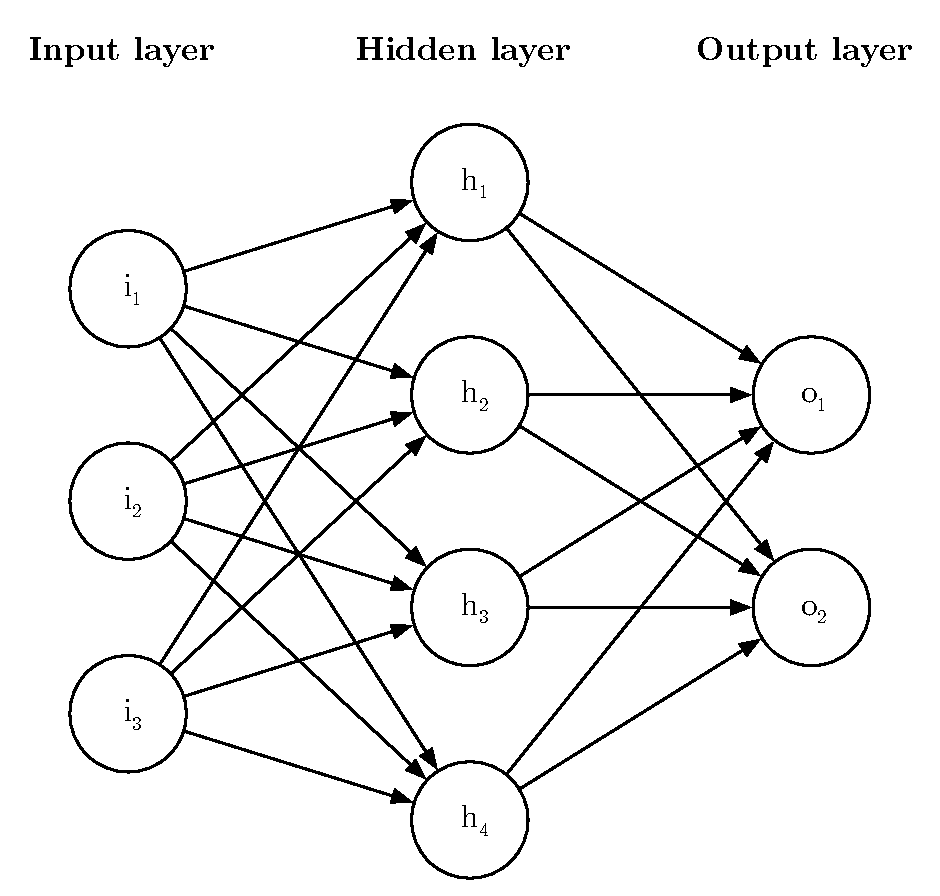
\includegraphics[width=0.6\linewidth]{fig/neural_network.eps}
	\caption{A neural network with one input layer composed of three neurons,
	one hidden layer of 4 neurons, and one output layer with 2 neurons.}
	\label{fig:neural_network}
\end{figure}


\section{Recurrent neural networks}
In some cases, it is a good idea to add a feedback loop to a neural network. 
A feedback loop such as the one shown in Figure~\ref{fig:rnn}, also called
a recurrent connection, poses evident issues for the backpropagation algorithm
since the depth of the neural network can become theoretically infinite.\\

A common way of training recurrent neural networks is to unroll them for a 
given, finite amount of time steps. The error signal can then be computed
for the output value at each time step, and backpropagated through all the
previous input values that affected its computing.\\

Recurrent neural networks are very useful in the context of reinforcement 
learning because they lay the ground for the memory aspect needed to solve
some tasks.

\begin{figure}[]
	\centering
	\subfloat[][A recurrent connection]{\qquad
		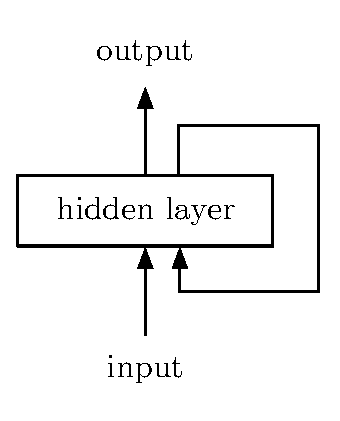
\includegraphics[width=0.1515\linewidth]{fig/recurrent_neural_network.eps}\qquad}
	\qquad
	\subfloat[][An unrolled recurrent neural network]{
		\includegraphics[width=0.6\linewidth]{fig/recurrent_neural_network_unrolled.eps}}
	\caption{Recurrent neural networks}
	\label{fig:rnn}
\end{figure}

\todo{universal function approximators}


